\documentclass[border=1mm]{standalone}
\usepackage{tikzlings}

\newcommand*{\pa}[1]{\coati[rotatehead=-10,santa=red,xshift=#1,book={\raisebox{-6mm}{\textcolor{black}{\sffamily\huge 1}}},bookcolour=gray!30!white]}
\newcommand*{\pb}[1]{\bear[graduate=black,tassel=yellow!70!red,xshift=#1,book={\raisebox{-6mm}{\textcolor{black}{\sffamily\huge 2}}},bookcolour=gray!30!white]}
\newcommand*{\pc}[1]{\sheep[xshift=#1,book={\raisebox{-6mm}{\textcolor{black}{\sffamily\huge 3}}},bookcolour=gray!30!white]}
\newcommand*{\pd}[1]{\penguin[crown=yellow!80!orange,xshift=#1,book={\raisebox{-6mm}{\textcolor{black}{\sffamily\huge 4}}},bookcolour=gray!30!white]}
\newcommand*{\pe}[1]{\owl[xshift=#1,book={\raisebox{-6mm}{\textcolor{black}{\sffamily\huge 5}}},bookcolour=gray!30!white]}

% 3 5 2 1 4    2 1
% 5 2 1 3 4    3 1
% 1 3 4 5 2    2 3
% 1 2 3 4 5    

\begin{document}
	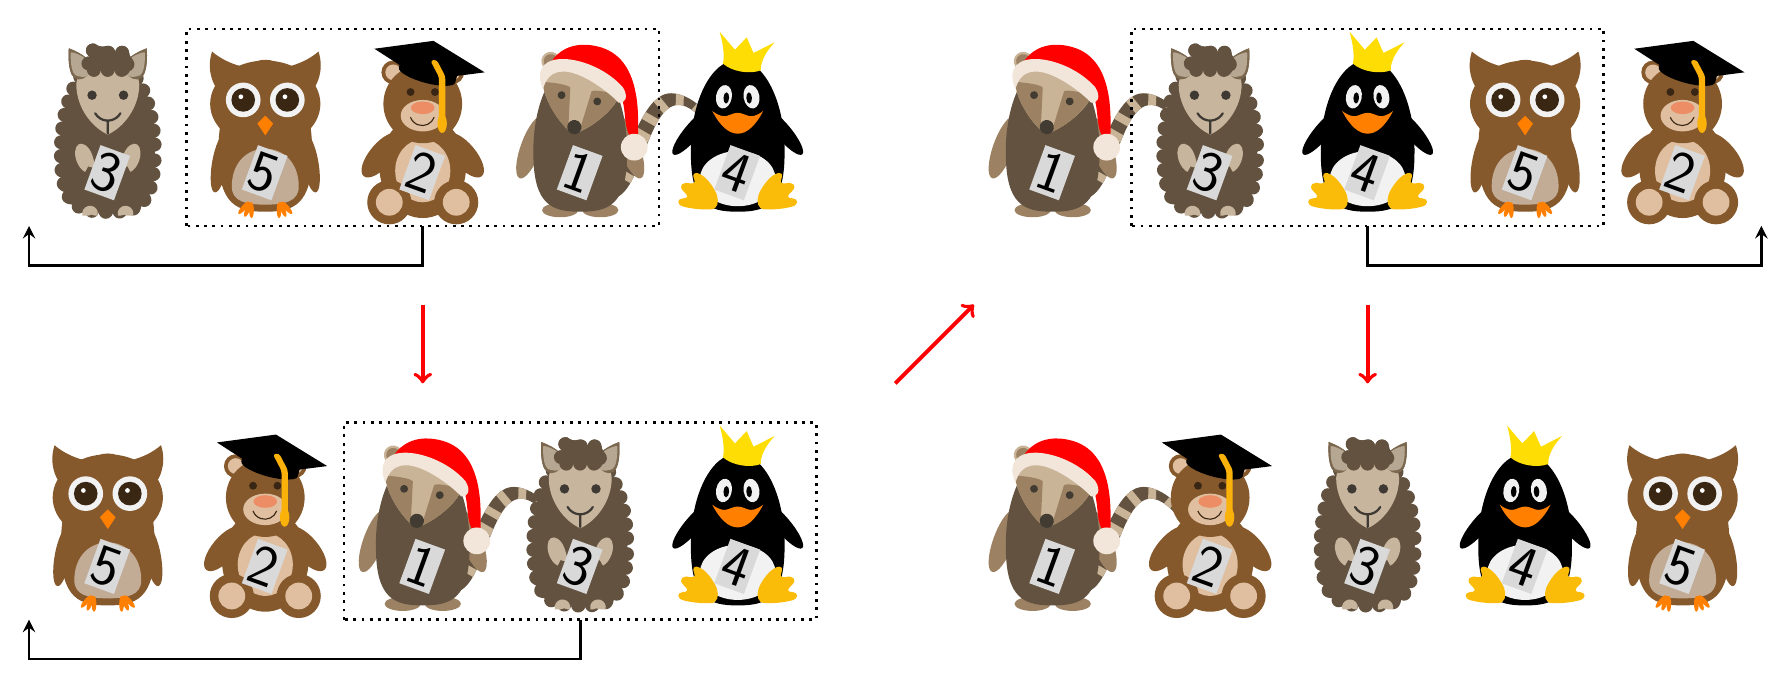
\begin{tikzpicture}[line width=0.35mm]
    \begin{scope}
      \pa{6cm} \pb{4cm} \pc{0cm} \pd{8cm} \pe{2cm}
      \draw[dotted] (1cm,0cm) rectangle (7cm,2.5cm);
      \draw[-stealth] (4cm,0cm) -- (4cm,-5mm) -- (-1cm,-5mm) -- (-1cm,0cm);
    \end{scope}
    \begin{scope}[yshift=-5cm]
      \pa{4cm} \pb{2cm} \pc{6cm} \pd{8cm} \pe{0cm}
      \draw[dotted] (3cm,0cm) rectangle (9cm,2.5cm);
      \draw[-stealth] (6cm,0cm) -- (6cm,-5mm) -- (-1cm,-5mm) -- (-1cm,0cm);
    \end{scope}
    \begin{scope}[xshift=12cm]
      \pa{0cm} \pb{8cm} \pc{2cm} \pd{4cm} \pe{6cm}
      \draw[dotted] (1cm,0cm) rectangle (7cm,2.5cm);
      \draw[-stealth] (4cm,0cm) -- (4cm,-5mm) -- (9cm,-5mm) -- (9cm,0cm);
    \end{scope}
    \begin{scope}[xshift=12cm,yshift=-5cm]
      \pa{0cm} \pb{2cm} \pc{4cm} \pd{6cm} \pe{8cm}
    \end{scope}
    \draw[->,red,line width=0.5mm] (4cm,-1cm) -- (4cm,-2cm);
    \draw[->,red,line width=0.5mm] (10cm,-2cm) -- (11cm,-1cm);
    \draw[->,red,line width=0.5mm] (16cm,-1cm) -- (16cm,-2cm);
	\end{tikzpicture}
\end{document}
